\documentclass[convert]{standalone}

\usepackage{tikz}
\pagestyle{empty}

% INT_AY22_L03_Fig05_Accel_ball.png

\begin{document}
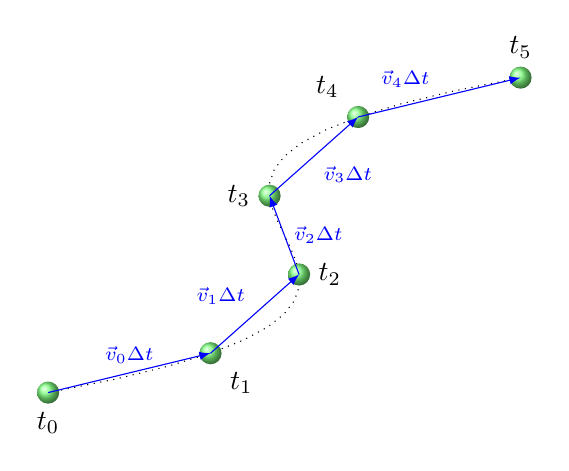
\begin{tikzpicture}[> = latex]

	% Curved path of motion

	\draw [domain = 0:4, variable = \y, dotted] plot ({0.5 * (\y - 1) * (\y - 2) * (\y - 3)}, \y);
	
	% Position of ball at various times
	
	\foreach \t/\Q/\n in {0/270/0, 0.5/315/1, 1.5/0/2, 2.5/180/3, 3.5/135/4, 4/90/5}
		\draw [ball color = green!50, draw = none] ({0.5 * (\t - 1) * (\t - 2) * (\t - 3)}, \t) circle (4 pt) node [label = {\Q : $t_\n$}] {};
		
	% Displacement vectors
		
	\foreach \ti/\tf/\n/\Q in {0/0.5/0/above, 0.5/1.5/1/above left, 1.5/2.5/2/right, 2.5/3.5/3/below right, 3.5/4/4/above left}
		\draw [blue, ->] ({0.5 * (\ti - 1) * (\ti - 2) * (\ti - 3)}, \ti) -- node [midway, font = \scriptsize, \Q] {${\vec v}_\n \Delta t$}
			({0.5 * (\tf - 1) * (\tf - 2) * (\tf - 3)}, \tf);
	
\end{tikzpicture}
\end{document}